
Figure \ref{pipeline} summarizes the general methodology that will be discussed. We will focus
on three main components, Data collection, Data processing and Data exploration.

\ \\ 
\noindent
\begin{tabular}{@{}cc}
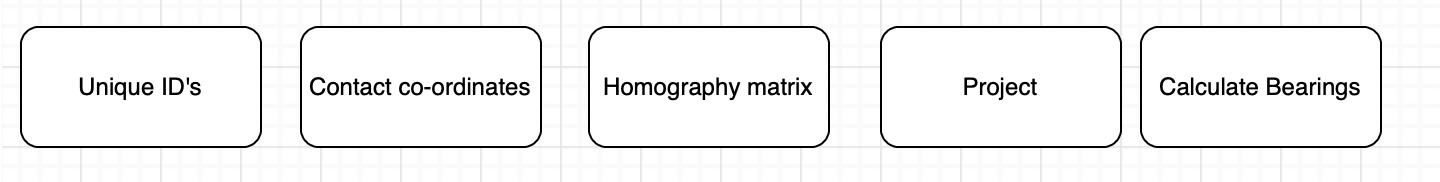
\includegraphics[width=1.0\columnwidth]{temp.png} 
\end{tabular}
\captionof{figure}{Data pipeline overview} 
\label{pipeline}

\subsection{Data Collection}

The Yrsas Plads junction in Copenhagen was chosen as the location for our primary data collection. 
This junction faces several challanges producing “conflicts, unsafe situations, illegal road user behaviour and great dissatisfaction among road users at the intersection” \cite{CPHpost_2021}.
These challenges make the Yrsas Plads junction one of the more complicated junctions in Copenhagen and would serve as a good base to this quantitative analysis method. 
As this is a large junction we have implmented a two cameras recording setup on opposite side of the junction, this provides good coverage regardless of traffic obstructions.

\subsubsection{Recording Location}

There are three consideration to take into account when applying these methods to a junction.
\begin{itemize}
	\item Junction size
\end{itemize}
Larger junctions would require a two camera setup as detailed, but this might not be optimal for intersections much Larger
than the Yrsas Plads junction. A larger junction might require more cameras which will need some implmentation tweeks.
\begin{itemize}
	\item Camera mounting points
\end{itemize}
\begin{itemize}
	\item Junction composition
\end{itemize}

\subsubsection{Camera Selection}

Modern mobile phones offer high resolution and quality cameras in a compact design. We used an LG G6 and a Samsung S7 Edge for recording the junction.
These devices offer wide enough field-of-views (FOV) to record the parts of the junction we are interested in from the selected mounting locations.
FOV being the maximum area a camera can image. A formal method of selecting a recording device would be to select one that has a large enough FOV that can image the entire junction 
from the mounting position that is closest to the junction. Given a recording location we can calculate the FOV needed using equation \ref{eq:1}.
If $\theta > FOV$ then the FOV is too small.
\begin{equation}
    \theta = tan^-1(\frac{\frac{width}{2}}{adjacent}) * 2\label{eq:1}
  \end{equation}

\ \\ 
  \begin{figure}[h]
    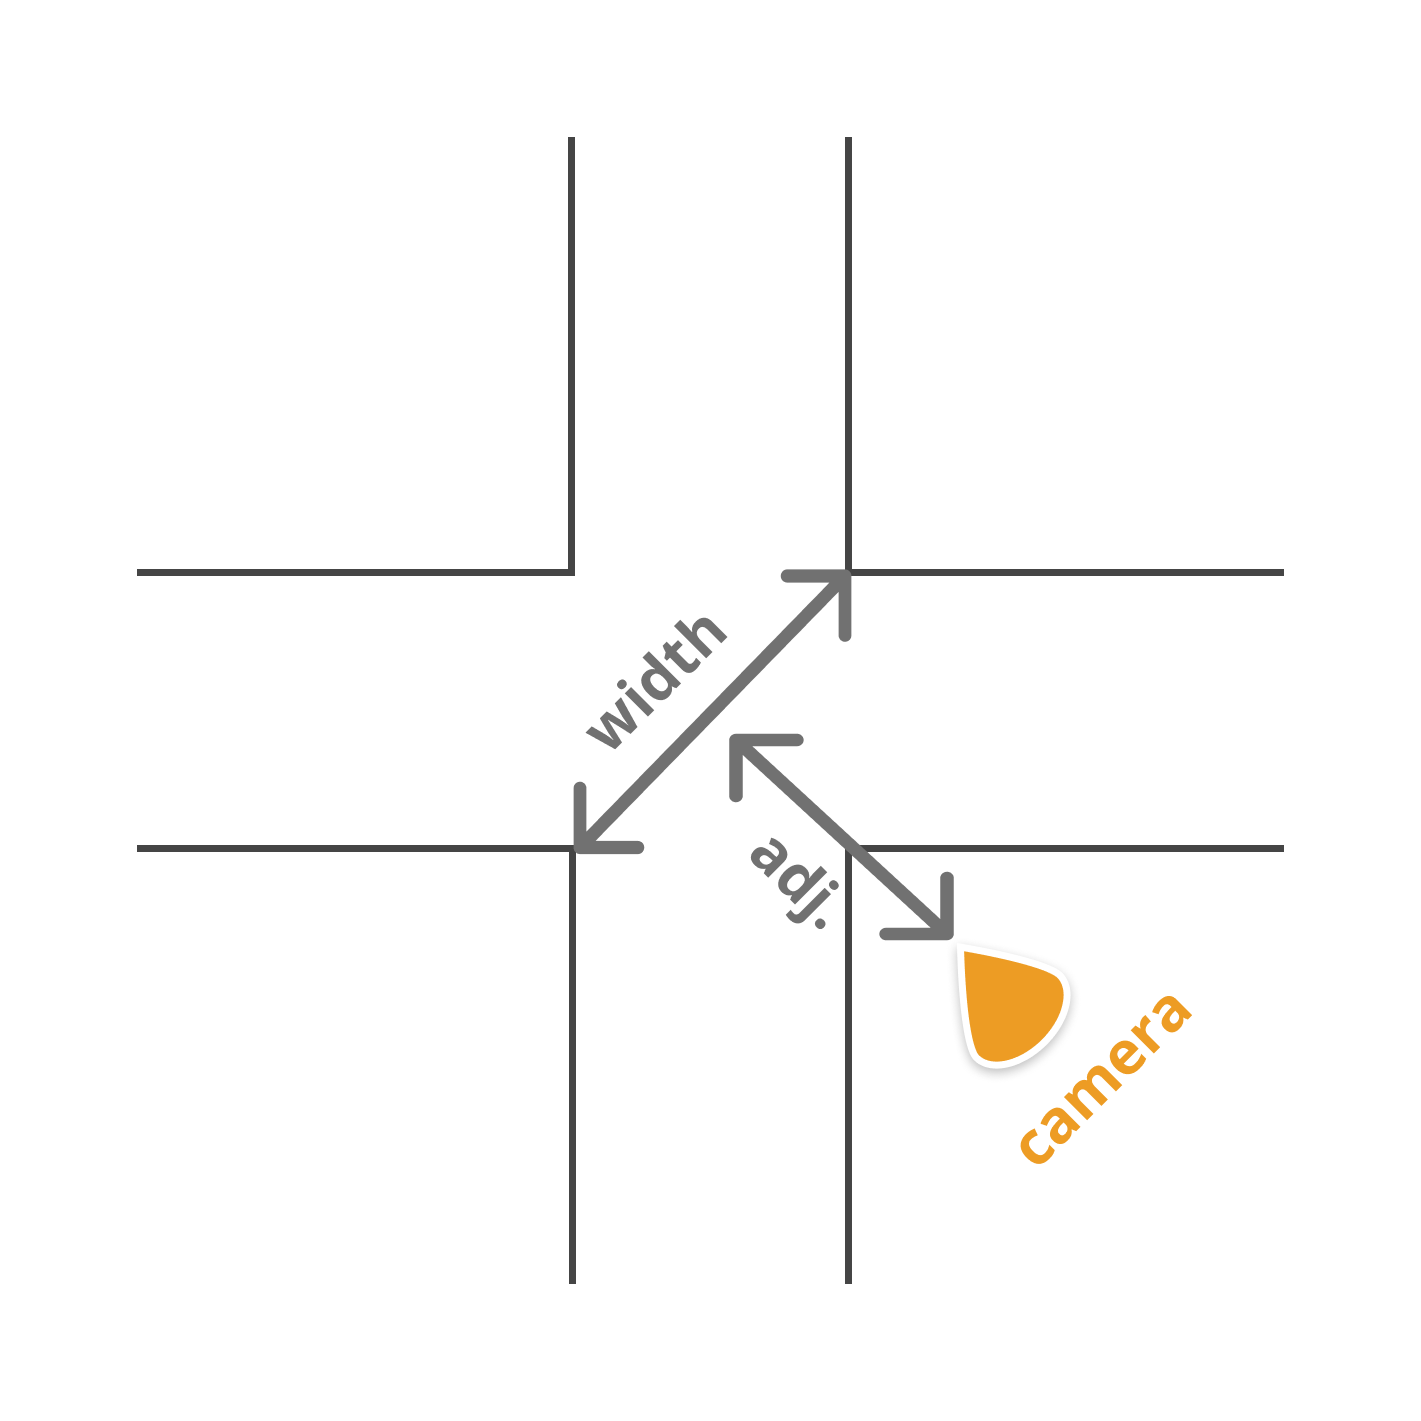
\includegraphics[scale=1.0]{location.png}
    \centering 
    \end{figure}
    \captionof{figure}{Barrel Distortion}
    \label{Camera location}

Battery life and storage capacity should also being considered depending on the amount of intended recording. 
With regards to storage 149MB per 1 min at 30FPS

\subsection{Data Processing}

\ \\ 
\noindent
\begin{tabular}{@{}cc}
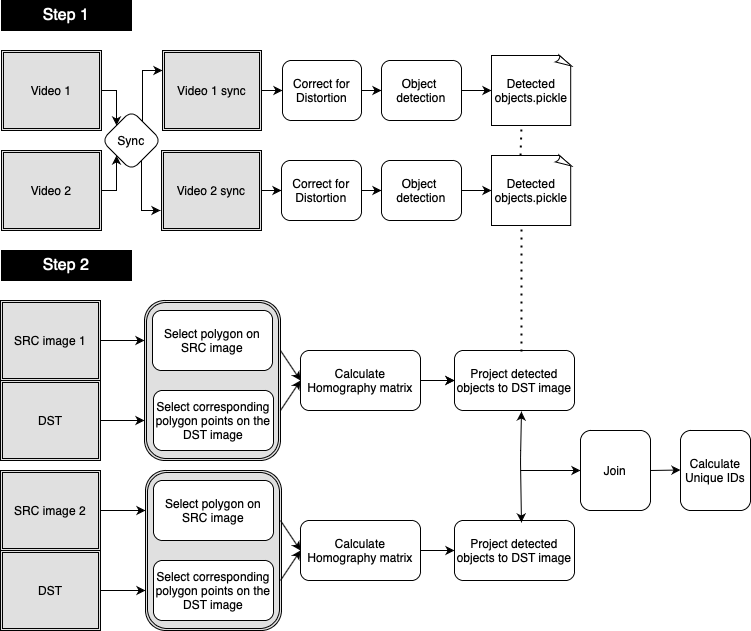
\includegraphics[width=1.0\columnwidth]{data_flow.png} 
\end{tabular}
\captionof{figure}{Data Pipeline}
\label{data}


Figure \ref{data} offers a general overview of the data processing steps. No special hardware is required, but a CUDA enabled GPU
device would speed up the object detection process.
\ \\
\subsubsection{Distortion Correction}

Wide angle camera lenses such as that on the LG G6 used in this study produce images that have an optical aberration where straight lines appear bent. 
The specific type being barrel distortion such as in figure \ref{distortion}, where lines curve inwards in a shape of a barrel.

\ \\ 
\begin{figure}[h]
  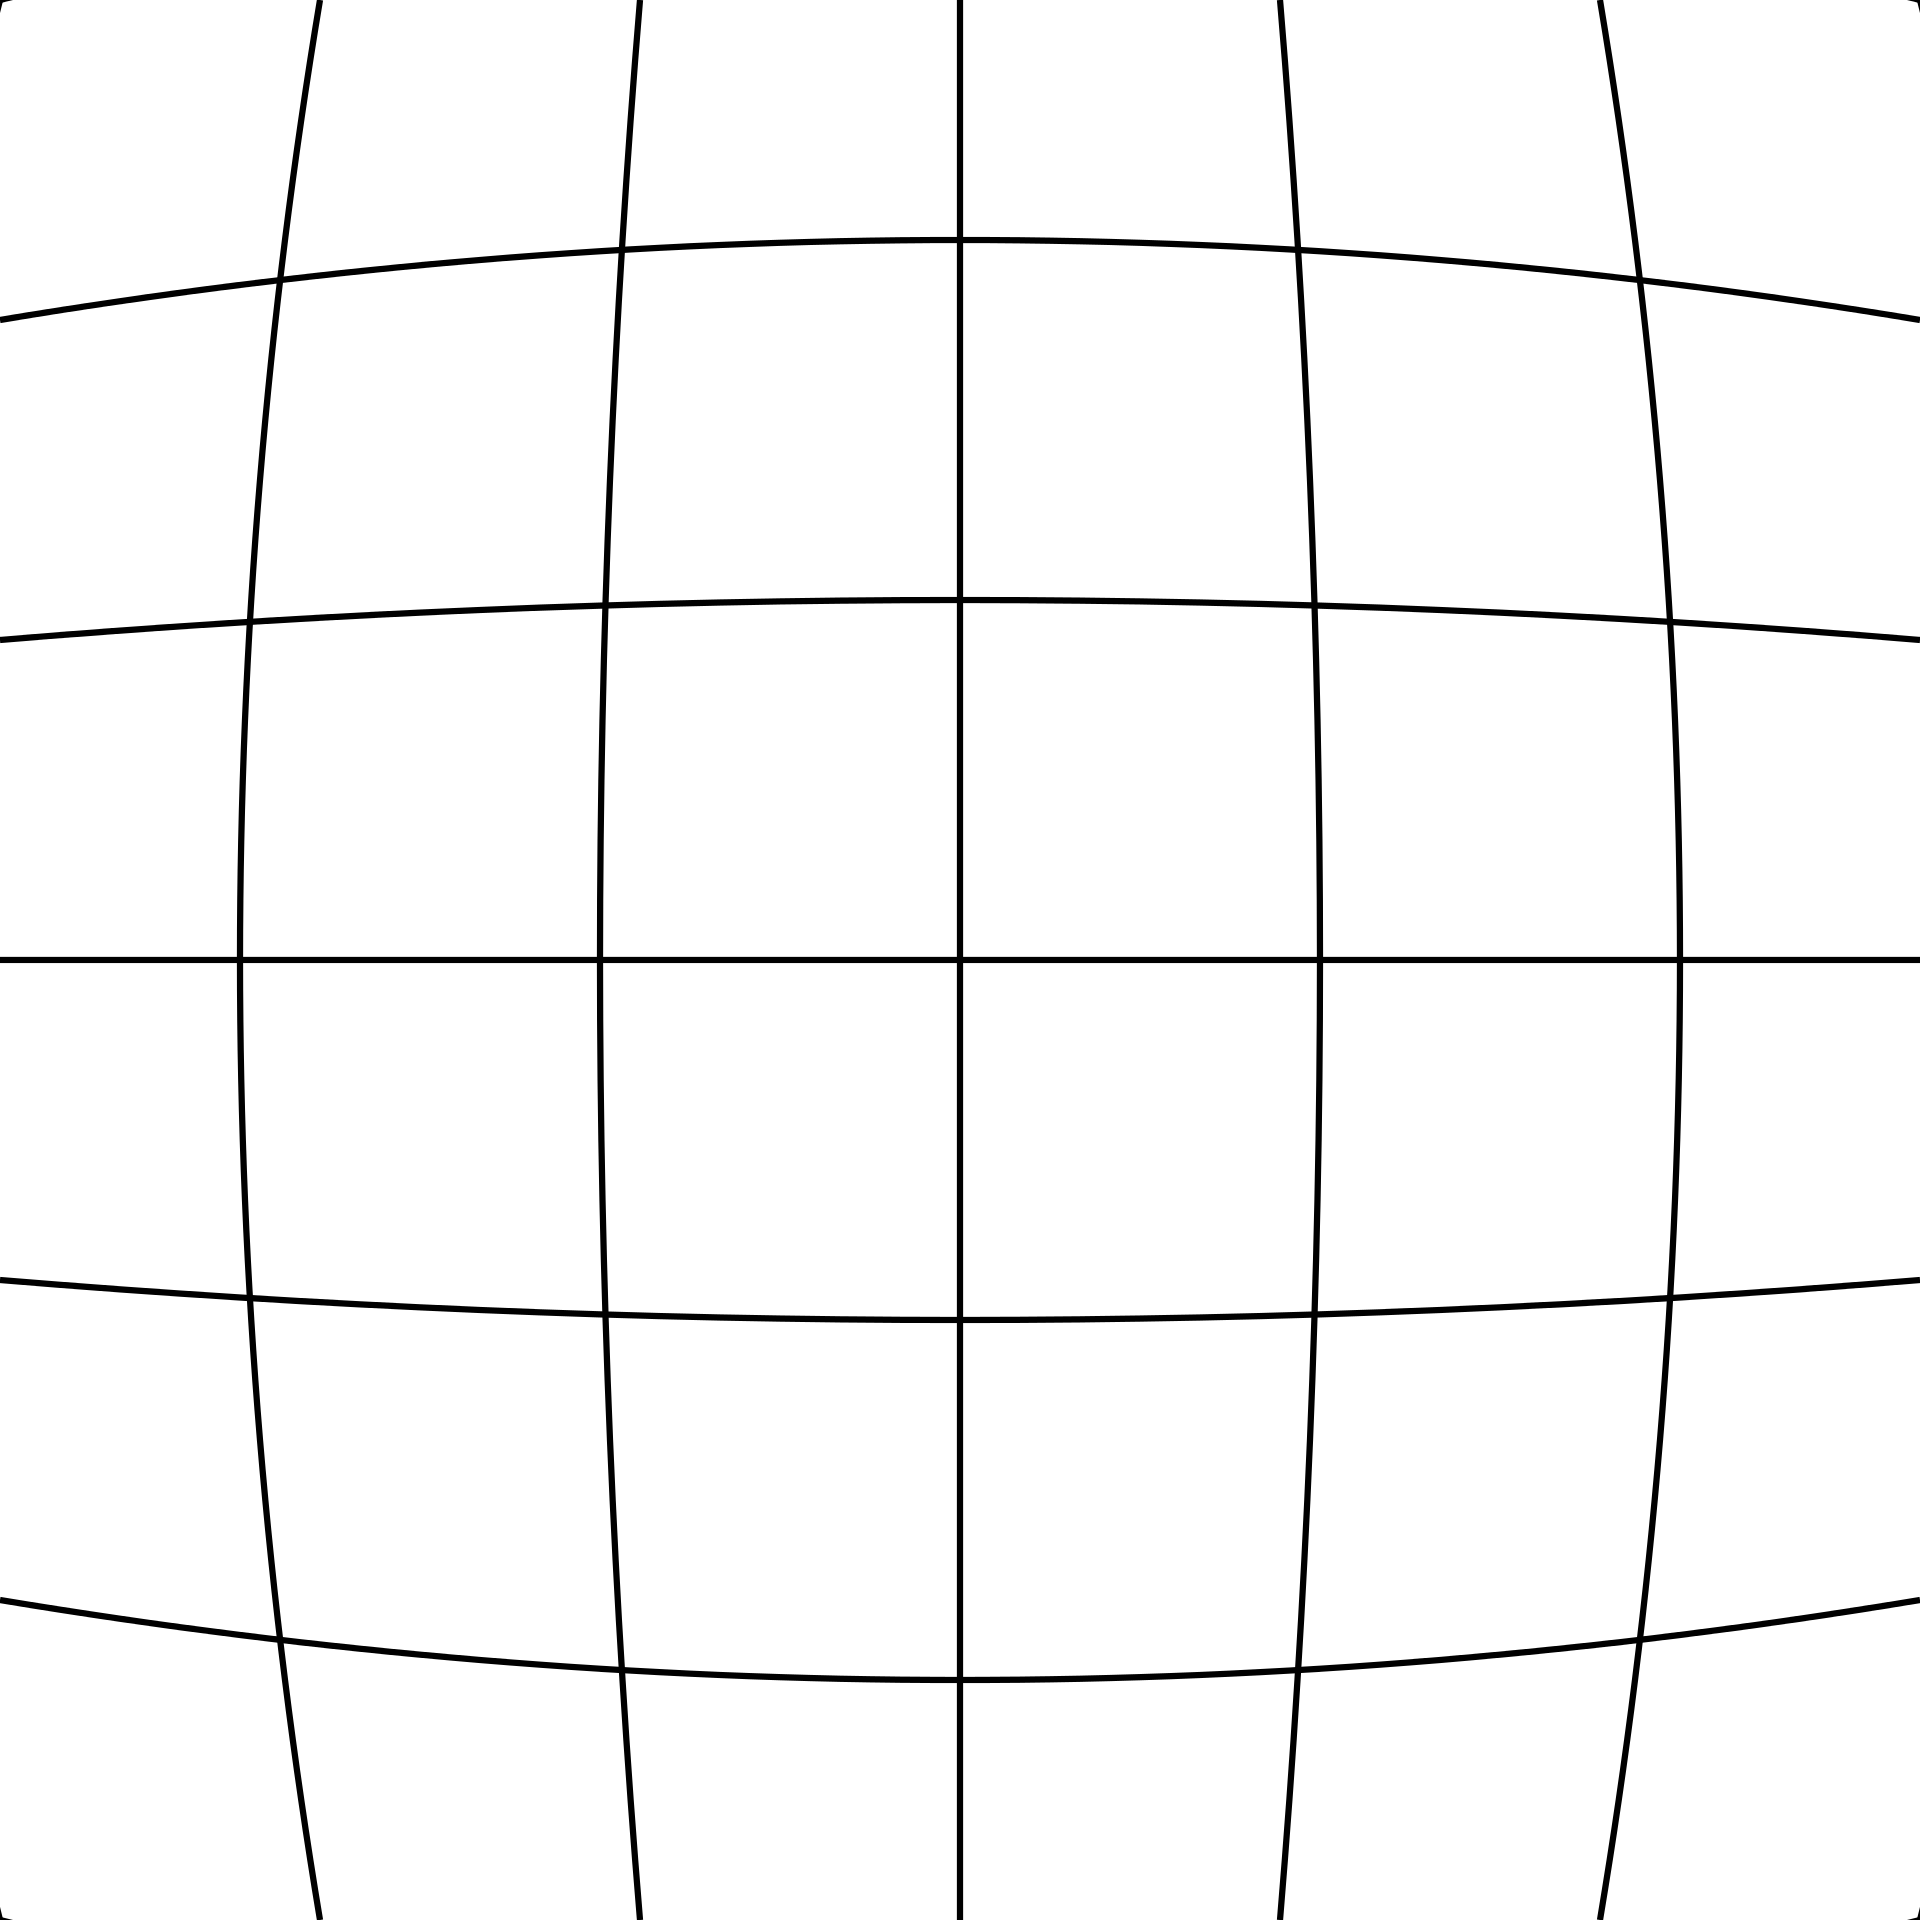
\includegraphics[scale=0.05]{Barrel_distortion.svg.png}
  \centering 
  \end{figure}
  \captionof{figure}{Barrel Distortion}
  \label{distortion}

\ \\
This can lead to incorrect projection and therefore joining of video sources later on.
To correct for this we make use of OpenCVs \cite{noauthor_opencv/opencv_2021} camera calibration toolbox.

Explain this a bit more. Formulas
\ \\
\subsubsection{Object Detection}

The raw video is output as a .mp4 file this video file is if fed to YOLO v5 for object detection. YOLO, You Only Look Once,
is a real-time object detection algorithm. ....Explain more.... 
\ \\ 
Why YOLO v5?
\ \\ 
Objects are detected each frame and represented as bounding boxes.
The output from YOLO is as follows: \[ [frame id][xmin][ymin][xmax][ymax][confidence]  \]

The min and max values for x and y represent a bounding box for the identified bicylce.

Figure \ref{data_pipeline} demonstrates the data pipeline that the output from YOLO is fed through. .
\ \\
\subsubsection{Homography Matrix}

First explain the concept of the homography matrix.
\ \\ 
\begin{figure}[h]
  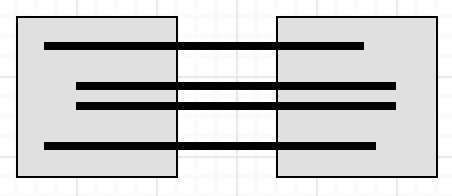
\includegraphics[scale=1.0]{Homography_proj.png}
  \centering 
  \end{figure}
  \captionof{figure}{SR to DST}
  \label{homography}

To transform the data to onto the a new plane view we needed to find the homography matrix, which is a transformation matrix between two planes \cite{hartley_zisserman_2004}.
The homography matrix (H) is a 3×3 matrix with 8 degrees of freedom, this allows the transformation of the cycling objects $P(x_r, y_r)$ to a 
top-down aerial view $P(x_i, y_i)$. The top-down view being an aerial image of the Yrsas Plads junction and P being the image coordinates in pixel units.

\begin{equation}
  P = HQ\label{eq:2}
\end{equation} 

\begin{align}
\label{eq:3}
  \begin{bmatrix}
    x_{i} \\
    y_{i} \\
    z_{i} \\
  \end{bmatrix}
  &= \begin{bmatrix}
      h_1 & h_2 & h_3 \\
      h_4 & h_5 & h_6 \\
      h_7 & h_8 & h_9 \\
  \end{bmatrix}
  \begin{bmatrix}
    x_{r} \\
    y_{r} \\
    z_{r} \\
  \end{bmatrix}
\end{align}
\subsubsection{Projection}

After finding the homography matrix we can now project to contact points of the bicycle and the road surface onto the destination
image being an aerial view of Yrsas Plads. This is achieved by applying $z$ to each point as a constant so as to create $Q(x_i, y_i, 1)$ and then we multipy it by 
homography matrix. 
\ \\
\subsubsection{Merging Sources}

To merge the data from the two video sources we take a naive approach. As the cameras are setup on
opposite siders of the junction for optimal coverage we simply cut the video sources in half along the halfway point between
the two cameras along the junction. The data is then merged.
\ \\
\subsubsection{Multiple object tracking}

In order to connect observations into trajectories of individual cyclist we apply 
simple online and real time tracking algorithm, SORT \cite{abewley_abewley/sort_2021}, as initially described in \cite{Bewley2016_sort}. 
SORT aims to address the problem of multiple object tracking (MOT) where object across frames needs to be connected. 
Explain more about SORT predict bbox then iou for actualy bbox.

The algorithm returns the bounding boxes along with a unique ID associated with each observation.

Using the bounding boxes we calculate the (x, y) co-ordinates of the observation and shift the y value down onto 
the same plane as the street so as to have the conact point of a bicycles and the street.

\subsection{Data Exploration}

There are two objectives for the data exploration.
\begin{itemize}
	\item1. Rainbow Tracks - Desire path discovery
	\item2. Alert Zones - For behaviour observations and counts
\end{itemize}

\subsubsection{Rainbow Tracks}

\ \\ 
\noindent
\begin{tabular}{@{}cc}
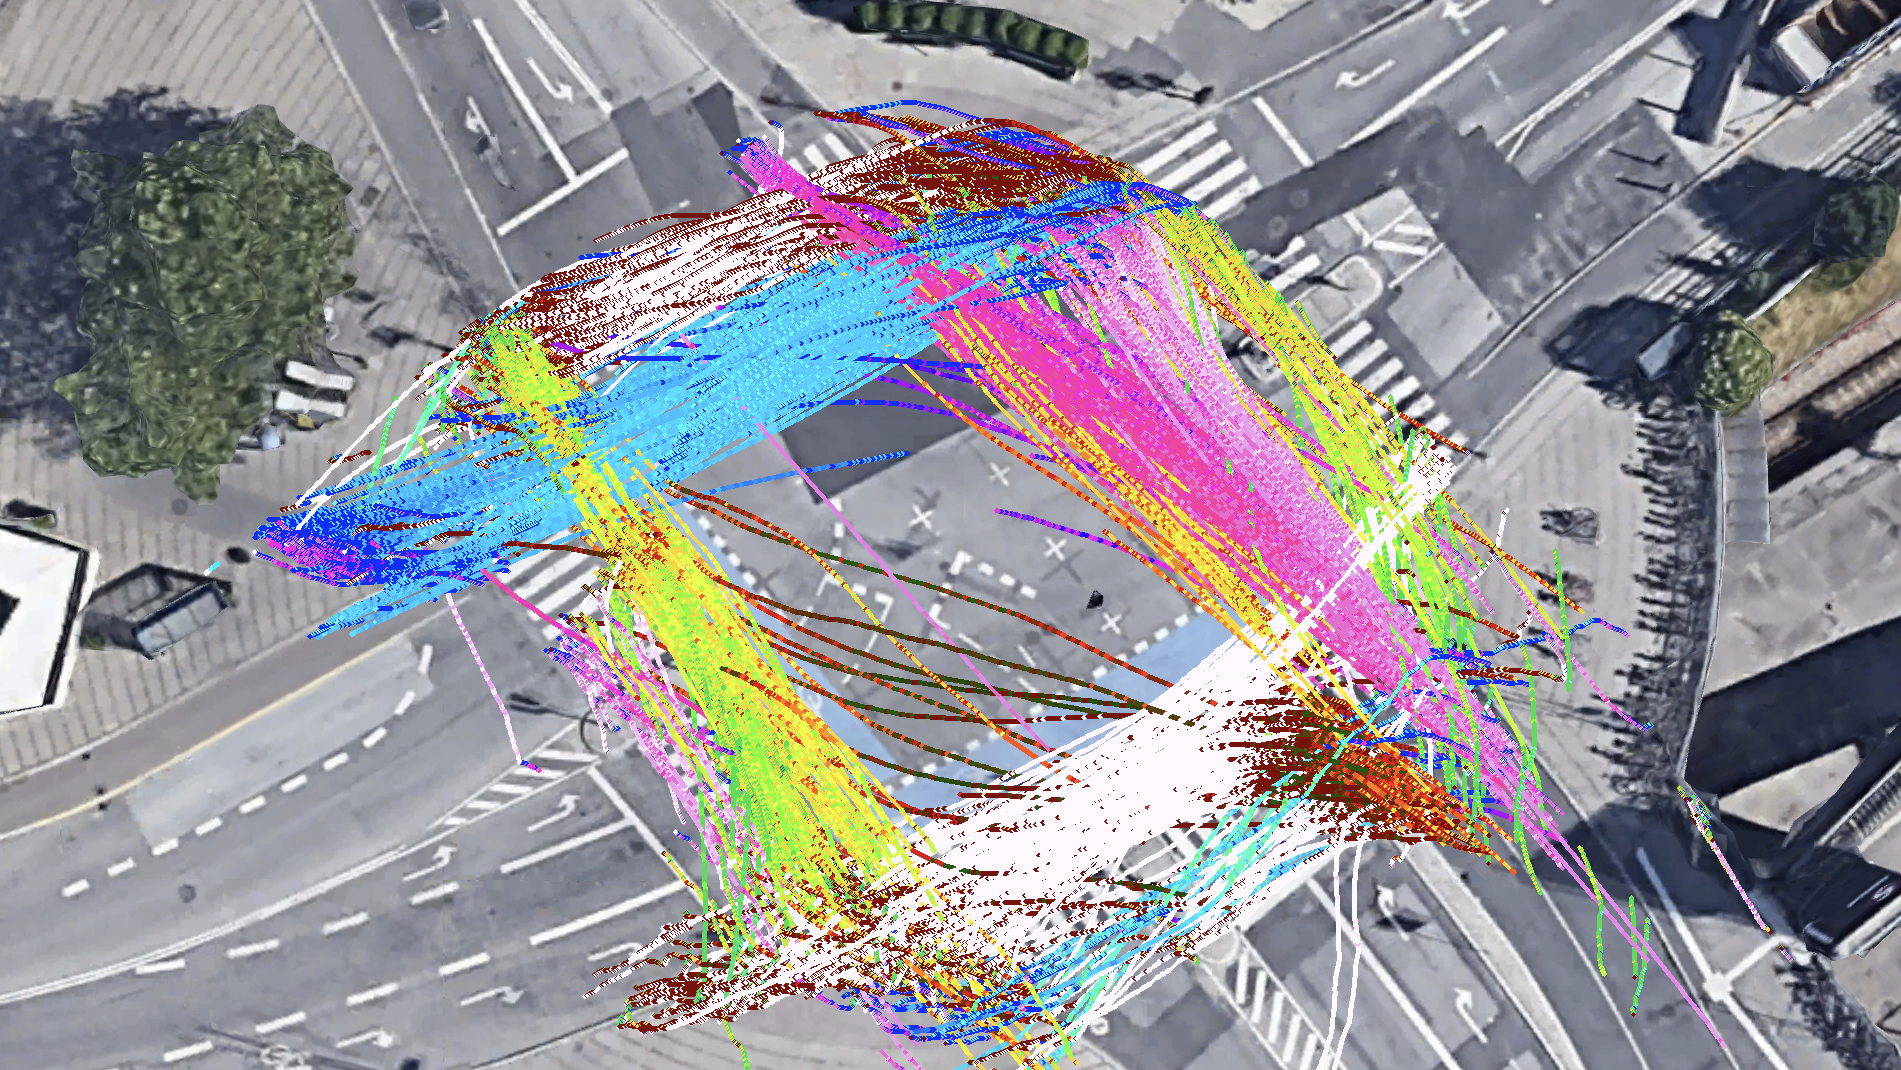
\includegraphics[width=1.0\columnwidth]{rainbow.png} 
\end{tabular}
\captionof{figure}{Rainbow}
\label{Rainbow}

To find aggregated desire lines from the data we took an approach which we call "Rainbow tracks". This involves coloring tracks by the bearing between consequtive points in each 
trajectory, after calculating the bearing we then get a color from a gardient color wheel. This approach has the added benefit of encoding direction into 
each track.
Maybe just an equation demonstaring the bearing calculation.
\ \\ 
\begin{equation}
  UniqueID_i = [(x_1, y_1)...(x_a+1, y_a+1)]\label{eq:3}
\end{equation}

\subsubsection{Alert Zones and Counts}

We created a "Tool name", that allows the defining of certain areas as "Red zones". These zones are provide us with easy reference to activty in the zones throught the videos.
Using these zones we can count cyclist and observe their behaviour at points on the junction that might be difficult or
problematic.

Picture of interface?
